\documentclass[12pt]{article}

\usepackage{amsmath}
\usepackage{graphicx}
\usepackage{hyperref}
\usepackage[latin1]{inputenc}
\usepackage{geometry}
\usepackage{graphicx}
\usepackage{titlesec}
\usepackage{pagecolor}

\geometry{tmargin=0.3in,bmargin=0.3in,lmargin=0.4in,rmargin=0.4in}

\titlespacing*{\section}{0pt}{1.1\baselineskip}{\baselineskip}

\title{\vspace{-2em}Report: Monthly Change in Value\vspace{-2em}}
\date{}

\begin{document}
\pagecolor{white}

\maketitle

\section{Problem Statement}
This report investigates the "ITE\_Data Assessment\_Dataset 1.csv" dataset. The purpose of this report is to uncover and discover any possible patterns of month over month change in value by type, either long-term or short-term. 

\section{Methodology}
For each variable type, values were averaged by month, and change in mean value from the previous month was calculated. The distribution of change in mean value by month was plotted for each type.

\section{Findings}
A boxplot view shows that all three variable types have similar distributions with regard to change in average value by month: mean around 0, 25th percentile around -1, 75th percentile around 1, minimum around -4, and maximum around 4 (Figure 1).
\\

\begin{center}
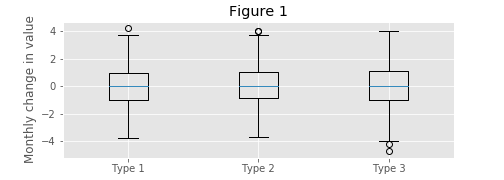
\includegraphics{figure.png}
\end{center}
Change in average value from month to month seems to be consistent, in that it doesn't seem to change very much based on time of year (Figure 2). This is the case for all three variable types.

\begin{center}
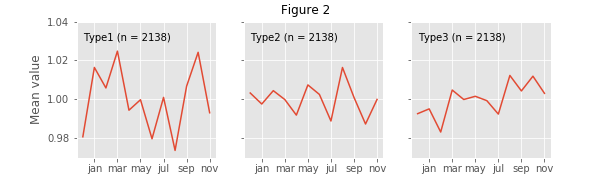
\includegraphics{subplot_figure.png}
\end{center}

\end{document}

    
    
    
\end{document}
